\documentclass[11pt,a4paper]{article}

\usepackage[margin=2.2cm]{geometry}
\usepackage[T1]{fontenc}
\usepackage{lmodern}
\usepackage{amssymb}
\usepackage{xcolor}
\usepackage{tikz}
\usetikzlibrary{arrows.meta,positioning}
\usepackage{booktabs}
\usepackage{tabularx}
\usepackage{enumitem}
\usepackage{listings}
\usepackage[most]{tcolorbox}
\usepackage{fancyhdr}
\usepackage[colorlinks=true,linkcolor=blue!50!black,urlcolor=blue!50!black]{hyperref}

\definecolor{local}{HTML}{2E7D32}
\definecolor{cloud}{HTML}{1565C0}
\definecolor{warn}{HTML}{C62828}
\definecolor{idea}{HTML}{6A1B9A}
\definecolor{soft}{HTML}{F5F5F5}
% sequential blue ramp (heatmap)
\definecolor{h0}{HTML}{EDEDEA}
\definecolor{h1}{HTML}{86B6EF}
\definecolor{h2}{HTML}{3987E5}
\definecolor{h3}{HTML}{256ABF}
\definecolor{h4}{HTML}{104281}

\newtcolorbox{concept}[1]{colback=idea!4,colframe=idea!70,fonttitle=\bfseries,title={Concept: #1},breakable}
\newtcolorbox{analogy}{colback=local!5,colframe=local!70,fonttitle=\bfseries,title={Analogy},breakable}
\newtcolorbox{why}{colback=cloud!4,colframe=cloud!70,fonttitle=\bfseries,title={Why it is done this way},breakable}
\newtcolorbox{caution}{colback=warn!4,colframe=warn!70,fonttitle=\bfseries,title={Watch out},breakable}
\newtcolorbox{exercise}{colback=soft,colframe=black!50,fonttitle=\bfseries,title={Check yourself},breakable}

\lstset{basicstyle=\ttfamily\small,backgroundcolor=\color{soft},frame=single,
        rulecolor=\color{black!25},columns=fullflexible,keepspaces=true,
        showstringspaces=false,breaklines=true}

\pagestyle{fancy}
\fancyhf{}
\lhead{\small Listen -- Learning Doc 08}
\rhead{\small The Web App}
\cfoot{\thepage}

\title{\textbf{Listen}\\[4pt]\large Learning Doc 08: The Web App\\
       \normalsize React, TypeScript, pages, data and charts}
\author{Detailed design, Section 7 (including the visual design)}
\date{17 October 2026, visual design added 18 October 2026}

\begin{document}
\maketitle

\begin{abstract}
\noindent This document designs the browser side of Listen: what a React app is, how
TypeScript keeps it in step with the server, how pages get their data, what each page shows,
and which chart answers which question, including the calendar heatmap. The last part records
the approved \emph{look}: two colour themes, Dock navigation, the React Bits components chosen
for each page, and the clickable prototypes in \texttt{docs/design/prototypes/} that serve as
the visual reference when the pages are built.
\end{abstract}

\tableofcontents
\newpage

% =====================================================================
\section{Decisions this section is built on}
\begin{center}
\renewcommand{\arraystretch}{1.2}
\begin{tabularx}{\textwidth}{l X}
\toprule
\textbf{Topic} & \textbf{Decision} \\
\midrule
Language     & \textbf{TypeScript}, with API types generated from the server. \\
Screens      & Laptop only. Pages are designed for a wide window (1280\,px and up); no phone layout. \\
Pages        & Login, Overview, History, App usage, Commands, Insights, Devices \& settings. Build order 1$\to$4 first. \\
Activity calendar & A calendar heatmap on Overview and Insights; darker = more commands (brighter in dark mode). \\
Visual design & Approved clickable prototypes (\S\ref{sec:visual}): Dock navigation, expressive React Bits components, light and dark themes. \\
From earlier & Talks only to the API (\texttt{/v1/\ldots}); refreshes every 5 minutes; guided form for command edits (Doc~07). \\
\bottomrule
\end{tabularx}
\end{center}

% =====================================================================
\section{What a React app is}

\begin{concept}{Single-page application (SPA)}
A traditional website asks the server for a whole new page on every click. A \textbf{single-page
application} loads \emph{once}: the browser downloads one bundle of JavaScript, which then draws
every page itself and only asks the server for \emph{data} (JSON from the API). Clicking from
Overview to History swaps what is on screen instantly, without reloading.
\end{concept}

\paragraph{An example: opening Listen, then clicking History.}
\begin{center}
\renewcommand{\arraystretch}{1.2}
\begin{tabularx}{\textwidth}{l X X}
\toprule
\textbf{Moment} & \textbf{Traditional website} & \textbf{Listen (SPA)} \\
\midrule
You open the site & Server sends a full Overview page (HTML) & Server sends one small HTML file + the app's JavaScript bundle (once); the app draws Overview, then fetches \texttt{/v1/analytics/summary} (JSON) \\
You click ``History'' & Browser throws the page away and downloads a full new History page; the screen flashes white & The app changes the address to \texttt{/history}, swaps the Overview component for the History component, fetches \texttt{/v1/analytics/commands} (JSON). No reload, no flash \\
You click ``Overview'' again & Another full page download & Overview's data is still in the cache (TanStack Query): it appears instantly \\
\bottomrule
\end{tabularx}
\end{center}
\noindent Gmail, Google Maps, Figma and Spotify's web player all work this way: after the first
load, only data travels.

\begin{concept}{Component}
React builds the screen out of \textbf{components}: functions that take some inputs and return
what to show. A page is a component made of smaller components (a stat tile, a chart, a table
row), the same way Listen's agent is made of small modules.
\end{concept}

\begin{lstlisting}[language=Java]
// web/src/components/StatTile.tsx   (TypeScript + JSX = "TSX")
type StatTileProps = { label: string; value: number; unit?: string };

export function StatTile({ label, value, unit }: StatTileProps) {
  return (
    <div className="stat-tile">
      <span className="label">{label}</span>
      <span className="value">{value}{unit}</span>
    </div>
  );
}

// used on the Overview page:
<StatTile label="Commands today" value={42} />
\end{lstlisting}

\noindent \texttt{label}, \texttt{value} and \texttt{unit} are the component's \textbf{props} (its
inputs); the \texttt{?} on \texttt{unit} means it is optional.

\begin{concept}{JSX, and how TypeScript turns it into TSX}
\textbf{JSX} lets you write HTML-looking tags \emph{inside} JavaScript. It is not HTML and the
browser cannot read it: before the app runs, the build tool (Vite) translates every tag into an
ordinary function call. This line
\begin{lstlisting}
<StatTile label="Commands today" value={42} />
\end{lstlisting}
becomes, roughly,
\begin{lstlisting}
jsx(StatTile, { label: "Commands today", value: 42 })
\end{lstlisting}
So a tag is just a neat way to call a component function with its props. Curly braces
\texttt{\{\ldots\}} mean ``this part is code, not text'': \texttt{value=\{42\}} passes the number 42,
\texttt{value="42"} would pass the text \texttt{"42"}.

A file of \emph{JavaScript} with JSX is \texttt{.jsx}; a file of \emph{TypeScript} with JSX is
\textbf{\texttt{.tsx}}. Same tags, but because the props have types, the tags are checked too:
\begin{lstlisting}
<StatTile label="Commands today" value="42" />
// error: Type 'string' is not assignable to type 'number'.
<StatTile label="Commands today" />
// error: Property 'value' is missing.                        (value is required)
\end{lstlisting}
TSX = JSX's convenient tags + TypeScript's checking of every tag's props.
\end{concept}

\begin{concept}{State and re-rendering}
\textbf{State} is data a component remembers and may change, such as which date range is
selected. When state changes, React runs the component again and updates only the parts of the
screen that changed. You never edit the page by hand; you change state and React redraws.
\end{concept}

% =====================================================================
\section{TypeScript in this app}

TypeScript adds type labels to JavaScript and checks them in the editor; before the browser
runs anything, the labels are removed. Its biggest job here is keeping the web app and the
server in agreement.

\begin{concept}{Generated API types}
FastAPI publishes a machine-readable description of every endpoint at \texttt{/openapi.json}
(the same data behind \texttt{/docs}). A tool (\texttt{openapi-typescript}) reads it and writes
\texttt{web/src/api/schema.ts}: a TypeScript type for every request and response. One command
regenerates it whenever the server changes. If a field is renamed on the server, every place in
the web app that uses the old name turns red, and the app will not build until it is fixed.
\end{concept}

\begin{lstlisting}[language=Java]
// generated from the server; never edited by hand
type CommandRow = components["schemas"]["CommandRow"];
//   { uuid: string; ts: string; heard: string; result: "executed" | "failed" | ... }

row.heared      // error: Property 'heared' does not exist. Did you mean 'heard'?
\end{lstlisting}

\begin{why}
Pydantic makes the \emph{server} reject bad data; the generated types make the \emph{web app}
unable to misread good data. The server's Python models become the single source of truth for
both halves, the same idea as \texttt{shared/recipe.schema.json} for commands (Doc~02).
\end{why}

% =====================================================================
\section{Project structure of \texttt{web/}}
\begin{lstlisting}
web/
|-- package.json        <- dependencies + scripts (npm run dev / build / test / gen:api)
|-- vite.config.ts      <- Vite: the dev server and build tool
|-- src/
|   |-- main.tsx         <- entry point: mounts the app into the page
|   |-- App.tsx          <- routes: which URL shows which page
|   |-- api/             <- schema.ts (generated) + client.ts (one place that calls fetch)
|   |-- pages/           <- one file per page: Overview.tsx, History.tsx ...
|   |-- components/      <- reusable pieces: StatTile, DataTable, DateRangePicker ...
|   |-- charts/          <- CalendarHeatmap, TrendLine, AppBars ...
|   `-- styles/          <- colour tokens (light/dark) and base styles
`-- tests/
\end{lstlisting}

\begin{concept}{Vite}
\textbf{Vite} is the tool that runs the app while you develop (\texttt{npm run dev}: saves show up
in the browser instantly) and builds the final optimised files for deployment
(\texttt{npm run build}). It handles TypeScript out of the box.
\end{concept}

% =====================================================================
\section{Moving between pages, and staying logged in}

\begin{concept}{Client-side routing}
\textbf{React Router} maps URLs to pages inside the SPA: \texttt{/} is Overview,
\texttt{/history} is History, and so on. The address bar and the back button work as on any
website, but no page is fetched from the server.
\end{concept}

\noindent \textbf{Protected pages.} On start-up the app calls \texttt{GET /v1/auth/me}. If the answer
is 401 (not logged in), every page redirects to \texttt{/login}. After logging in, the session
cookie (Doc~07) does the rest; the web app never stores your password or the session id itself.

% =====================================================================
\section{Getting data: one cache for the whole app}

\begin{concept}{Server-state cache (TanStack Query)}
Data from the API is stored in one shared \textbf{cache}, managed by a library called
\textbf{TanStack Query}. A component says ``I need \texttt{/v1/analytics/apps} for this week'';
the library fetches it once, shares it with every component that asks for the same thing,
refreshes it every 5 minutes (the decided refresh rate), and refreshes when you come back to the
tab. Each request is in one of three states, and every page designs all three:
\textbf{loading}, \textbf{error}, or \textbf{data}.
\end{concept}

\noindent \textbf{The sleeping server.} If the first request takes longer than 3 seconds, the
loading state changes to ``Waking up the server\ldots (this can take up to a minute on the free
tier)'' instead of an endless spinner.

\noindent \textbf{One date range.} A date-range control at the top of each analytics page (today,
last 7 / 30 / 90 days, custom) drives every chart on that page together.

% =====================================================================
\section{The pages}

\subsection{1. Login}
Username, password, ``Log in''. Wrong password: one generic message (``Username or password is
incorrect'') that never reveals which one was wrong. Lock-out (Doc~07): ``Too many attempts. Try
again in 15 minutes.''

\subsection{2. Overview, ``today at a glance''}
\begin{itemize}[nosep]
  \item The \textbf{``Listen'' title} with a one-line summary (commands today, \% understood), and
        the \textbf{activity calendar} beside it.
  \item \textbf{Stat cards}: commands today, success rate today, top app today, median response
        time, top site, no-match count, streak; each with its change versus the previous 7-day
        average.
  \item The last 8 commands (what was heard; hover shows the command, result and response time).
        Clicking one opens it in History.
  \item Laptop status: ``Last synced 3 minutes ago'' (from \texttt{GET /v1/devices}).
\end{itemize}

\subsection{3. History}
Every command, newest first, 50 per page, with search on the heard text and filters (result,
mode, command, date range). Each row can be marked \emph{right} / \emph{wrong} or deleted
(Doc~07), with a confirmation for delete.

\subsection{4. App usage}
Time per app for the selected range, time per site inside a chosen app (Chrome $\to$ Google Search,
YouTube \ldots), and how daily time changed over the range.
\begin{itemize}[nosep]
  \item \textbf{Top 7 + ``Other''} as bars: the quick summary. ``Other'' is clickable.
  \item \textbf{Every app}: a searchable, sortable list of \emph{all} apps (time, share of total,
        change versus the previous period, days used). Selecting a row is the same as clicking a bar.
  \item \textbf{Trend}: one app highlighted with the others grey by default, or \textbf{compare up
        to 4 apps}, each with its own colour \emph{and} marker shape and its name at the end of its
        line. A 5th pick waits until a colour is free; removing an app never repaints the others.
        Days an app was not opened are drawn dotted along zero (``0 min, not missing data'').
  \item The trend chart can be \textbf{zoomed in and out} (drag to select a stretch of days, reset
        to the full range), so four lines over 90 days stay readable.
\end{itemize}
The server already returns every app (Doc~07), so none of this changes the API.

\subsection{5. Commands}
Your commands and routines as cards grouped by file (\texttt{core}, \texttt{browser},
\texttt{routines} \ldots), read from the latest snapshot. ``Add'' and ``Edit'' open the guided form,
which submits a pending edit; a panel lists pending edits with their status (waiting for laptop /
applied / invalid / overridden).

\subsection{6. Insights}
The activity calendar, trends, sentences that did not match, latency, and calibration (charts
below).

\subsection{7. Devices \& settings}
Your laptop with its last sync time; create a new device token (shown once, with a copy button
and a clear warning that it will not be shown again); revoke; log out; and the theme choice
(Windows / Light / Dark), which is remembered in this browser.

% =====================================================================
\section{Charts: the right form for each question}

A chart is chosen by the \emph{job} the reader must do, before any colour is picked.

\begin{center}
\renewcommand{\arraystretch}{1.25}
\begin{tabularx}{\textwidth}{>{\raggedright\arraybackslash}p{4.6cm} >{\raggedright\arraybackslash}X >{\raggedright\arraybackslash}p{4.0cm}}
\toprule
\textbf{Question} & \textbf{Form} & \textbf{Colour job} \\
\midrule
How active was I each day this year? & Calendar heatmap & Sequential (one hue; darker = more in light mode, brighter = more in dark) \\
Am I using Listen more or less over time? & Line, commands per day & One series: one hue, no legend \\
Is Listen getting things right more often? & Line, success rate per day & One hue \\
Today's headline numbers & Stat tiles, not charts & Ink only; delta arrow + label \\
Which apps take my time? & Horizontal bars, top 7 + ``Other'' & One hue (it is magnitude, not identity) \\
How did one app's time change? & Line: that app highlighted, others grey & Emphasis: one hue + grey \\
How do a few apps compare? & Line, up to 4 apps, zoomable & Categorical, 4 slots + marker shapes, direct-labelled \\
Where does the 1.5\,s go? & Stacked bars per day, 4 stages, with a 1.5\,s reference line & Categorical, 4 slots, direct-labelled \\
Are low scores really the wrong guesses? & Two small histograms (right / wrong) with the threshold marked & Two categorical slots \\
Which sentences failed? & A table (not a chart) & Ink only \\
\bottomrule
\end{tabularx}
\end{center}

\subsection{The activity calendar}
\begin{center}
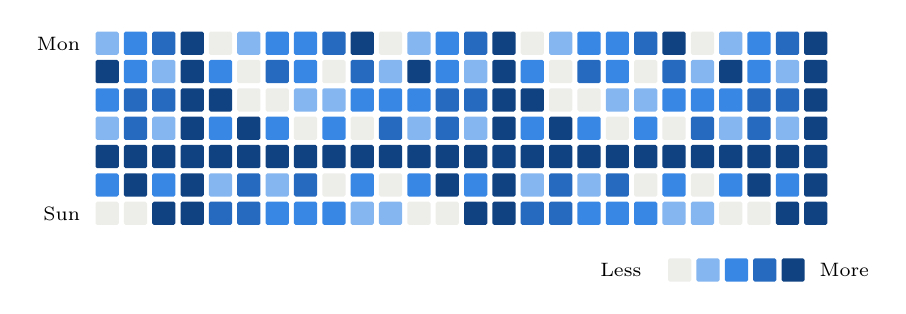
\begin{tikzpicture}[x=0.36cm,y=0.36cm]
  \foreach \w in {0,...,25} {
    \foreach \d in {0,...,6} {
      \pgfmathsetmacro{\v}{mod(\w*13+\d*7+\w*\d*5+3,11)}
      \ifdim\v pt<2pt \def\c{h0}\else\ifdim\v pt<4pt \def\c{h1}\else\ifdim\v pt<7pt \def\c{h2}\else\ifdim\v pt<9pt \def\c{h3}\else\def\c{h4}\fi\fi\fi\fi
      \fill[\c,rounded corners=0.6pt] (\w,-\d) rectangle ++(0.82,0.82);
    }
  }
  \node[font=\scriptsize,anchor=east] at (-0.2,0.4) {Mon};
  \node[font=\scriptsize,anchor=east] at (-0.2,-5.6) {Sun};
  \node[font=\scriptsize,anchor=east] at (19.6,-7.6) {Less};
  \foreach \c [count=\i] in {h0,h1,h2,h3,h4} \fill[\c,rounded corners=0.6pt] (19.2+\i,-8) rectangle ++(0.82,0.82);
  \node[font=\scriptsize,anchor=west] at (25.2,-7.6) {More};
\end{tikzpicture}
\\[2pt]{\footnotesize Illustration only (made-up data, 26 weeks shown); the real one shows 53 weeks.}
\end{center}

\begin{itemize}[nosep]
  \item One square per day, columns are weeks, rows are weekdays.
  \item \textbf{Light mode: darker = more commands that day} (decided). Days with no commands are a
        light grey square, so ``nothing'' never looks like ``a little''.
  \item \textbf{Dark mode: brighter = more} (decided). On a dark page, ``darker'' would mean
        ``closer to the background'', so the busiest days would almost vanish. Instead busy days
        glow: zero is a dark slate square (\texttt{\#2A3440}) and the 4 steps run
        \texttt{\#1C5CAB} $\to$ \texttt{\#2A78D6} $\to$ \texttt{\#5598E7} $\to$ \texttt{\#9EC5F4},
        starting one shade lighter than light mode because the darkest blue failed the 2:1
        contrast check against the dark surface. The rule in both modes: \emph{more activity =
        stands out more}.
  \item Days with commands fall into \textbf{4 blue steps} using \textbf{quartiles} of your own
        active days, so one unusually busy day does not make every other day look empty.
  \item Hovering a square shows the date and the exact count; a ``Less $\to$ More'' key sits
        underneath. Data comes from a new endpoint, \texttt{GET /v1/analytics/calendar?year=2026},
        returning one count per day.
\end{itemize}

\begin{concept}{Sequential vs.\ categorical colour}
\textbf{Sequential} colour shows \emph{how much}: one hue, light to dark (the calendar, app bars).
\textbf{Categorical} colour shows \emph{which one}: different hues for different things (the four
latency stages). Using many hues for ``how much'' makes people read categories that are not
there, so magnitude always uses one hue.
\end{concept}

\subsection{Rules every chart follows}
\begin{itemize}[nosep]
  \item \textbf{One y-axis per chart.} Two measures with different units get two charts, never a
        double-axis chart (the most common way charts mislead).
  \item \textbf{Hover tooltips} on every chart: exact value, date, and label.
  \item \textbf{Never colour alone}: two or more series always have a legend, and up to four are
        labelled directly on the chart; every chart can switch to a table view.
  \item \textbf{Text stays in text colours} (black/grey ink), never in a series colour.
  \item \textbf{Validated palette}: a tested colour-blind-safe palette, checked with a palette
        validator for both light and dark mode. Status colours (good / warning / error) are
        reserved and always come with an icon and a word.
  \item \textbf{Light and dark mode}, following Windows' setting unless you pick one, each with its
        own validated steps.
\end{itemize}

\paragraph{Tools.} \textbf{Recharts} (a React chart library) for lines and bars. The calendar
heatmap is a small custom component drawn in SVG: 371 squares is simple enough that a library
would add weight without adding value.

% =====================================================================
\section{Visual design}\label{sec:visual}

\subsection{How the look was chosen}
\begin{enumerate}[nosep]
  \item \textbf{Three directions on one screen} (in Figma): A ``Quiet Ledger'' (calm, light),
        B ``Signal Desk'' (dark instrument panel), C ``Soft Studio'' (warm, rounded). Same Overview,
        same data, so only the look differed.
  \item \textbf{Pick and combine}: A becomes light mode, B becomes dark mode (same layout).
  \item \textbf{Your redesign of Overview} with components you chose from React Bits, built as a
        clickable prototype, then \textbf{all seven pages} in the same language, with every state.
\end{enumerate}

\begin{concept}{Prototype: a picture that you can click}
A \textbf{prototype} is a fake version of the app that looks and behaves like the real one but
has made-up data and no server. Figma frames are still pictures, which is fine for layout but
useless for judging animation: a spiral of cards or a menu that flows on hover only makes sense
when it moves. So the pages were built as small web pages that run the real React Bits code.
They live in \texttt{docs/design/prototypes/}; open \texttt{index.html}.
\end{concept}

\subsection{Theme tokens}
\begin{center}
\renewcommand{\arraystretch}{1.15}
\begin{tabularx}{\textwidth}{l X X}
\toprule
 & \textbf{Light (A, Quiet Ledger)} & \textbf{Dark (B, Signal Desk)} \\
\midrule
Background / card & \texttt{\#F5F6F8} / \texttt{\#FFFFFF} & \texttt{\#131A22} / \texttt{\#18212B} \\
Text              & \texttt{\#1D2330}                     & \texttt{\#E6EBF2} \\
Accent            & \texttt{\#2A78D6}                     & \texttt{\#5598E7} \\
Fonts             & Instrument Sans                        & IBM Plex Sans; IBM Plex Mono for numbers and command ids \\
Corners           & 12\,px                                 & 8\,px \\
\bottomrule
\end{tabularx}
\end{center}
The theme follows Windows by default. The Windows / Light / Dark choice in the header and on
Devices \& settings overrides it and is \textbf{remembered in this browser}.

\begin{concept}{Design tokens}
A \textbf{token} is a named design value (\texttt{-{}-accent}, \texttt{-{}-surface},
\texttt{-{}-radius}) used everywhere instead of a raw colour or number. Components say ``use the
accent'', never ``use \texttt{\#2A78D6}''. Dark mode is then just a second set of values for the
same names, and changing the accent later is a one-line edit. This is also why the Dock could be
recoloured to match the page without touching its code: its colours were pointed at the page's
tokens.
\end{concept}

\subsection{Navigation and shared parts}
\begin{itemize}[nosep]
  \item \textbf{Dock} (React Bits) at the bottom instead of a sidebar: six pages plus Log out,
        names on hover, the current page's tile tinted with the accent. No badges. Login has no
        Dock, because you are not logged in yet.
  \item \textbf{Header}: the date, ``Last synced \ldots'', and the theme switch.
  \item \textbf{States on every page}: Loading (page-shaped placeholders), Waking up (the free
        server is starting; elapsed timer), Error (what failed, ``nothing is lost'', Try again),
        Empty (first day: example sentences and ``Connect your laptop'').
  \item \textbf{Hold to confirm}: deleting a command or revoking a device means holding a button
        down until it fills, instead of an ``Are you sure?'' dialog.
\end{itemize}

\subsection{Components per page}
\begin{center}
\renewcommand{\arraystretch}{1.15}
\begin{tabularx}{\textwidth}{l X}
\toprule
\textbf{Page} & \textbf{Main pieces (React Bits unless noted)} \\
\midrule
Login     & TechText ``Listen'', LineWaves background, SpecularButton, Counter for the lock-out countdown \\
Overview  & TechText ``Listen'' + activity calendar, InfiniteSpiral of stat cards, FlowingMenu of recent commands \\
History   & SplitFlapText title (a departure board), a real table with every column, GlideSelect filters, HoldButton delete \\
App usage & Counter total, top-7 bars, OptionWheel to pick an app, ``Every app'' list, compare up to 4 (SpringCheck boxes), zoomable trend \\
Commands  & Folder per command file, SpotlightCard per command, Stepper guided form, AnimatedList of pending edits \\
Insights  & MagicBento tiles, BlurText one-line takeaways, every chart with a Table view \\
Devices   & TearTicket + DecryptedText for the one-time token, HoldButton revoke, JellyRadio theme choice \\
\bottomrule
\end{tabularx}
\end{center}

\begin{why}
The interaction should \emph{mean} something. The device token is shown once, so it appears as a
ticket: the characters unscramble, and you tear off the stub to confirm you saved it, just as you
would keep a real ticket stub. History is a log of events, so its title flips like a departure
board. Deleting is permanent, so it needs a deliberate hold rather than a quick click. Dense data
(History, the every-app list) stays a plain table, because decoration must never make numbers
harder to read.
\end{why}

\begin{caution}
These pages animate continuously (TechText, the spiral). That uses some CPU while the web app is
open, which is acceptable because ``lightweight'' is a rule for the \emph{laptop agent}, and the
dashboard is only open when you choose to look at it. Every animation still stops when Windows
asks for reduced motion.
\end{caution}

% =====================================================================
\section{Testing the web app}
\begin{itemize}[nosep]
  \item \textbf{Type check} (\texttt{tsc}): the whole app must compile without type errors.
  \item \textbf{Component tests} with Vitest and React Testing Library: render a component with fake
        data and check what a user would see (``the calendar shows 371 squares'', ``a 401 sends you
        to the login page'').
  \item The API is \textbf{mocked} in these tests, so they run in seconds without a server.
\end{itemize}

% =====================================================================
\section{Glossary}
\begin{description}[style=nextline,leftmargin=1.2cm,itemsep=2pt]
  \item[Calendar heatmap] One square per day; darker means more (brighter in dark mode).
  \item[Component / props] A function that returns what to show / its inputs.
  \item[Design token] A named design value (colour, size) used instead of raw values.
  \item[Dock] A row of app-style icons for moving between pages.
  \item[Generated types] TypeScript types produced automatically from the server's API description.
  \item[JSX / TSX] HTML-like syntax inside JavaScript / TypeScript code.
  \item[Prototype] A clickable fake of the app with made-up data, used to judge the design.
  \item[Quartiles] Values splitting sorted data into four equal-sized groups.
  \item[React Router] Maps URLs to pages inside a single-page app.
  \item[Sequential / categorical colour] One hue for ``how much'' / different hues for ``which one''.
  \item[SPA] A web app that loads once and then only fetches data.
  \item[State] Data a component remembers; changing it redraws the component.
  \item[TanStack Query] A library that fetches, caches and refreshes API data.
  \item[Vite] The development server and build tool for the web app.
\end{description}

% =====================================================================
\section{Check your understanding}
\begin{exercise}
\begin{enumerate}
  \item What does the browser download once in an SPA, and what does it keep fetching after that?
  \item A field is renamed on the server. Walk through how the web app finds out.
  \item Why do days with zero commands get grey, not the lightest blue?
  \item Why are the calendar's blue steps based on quartiles of \emph{your} days rather than fixed
        numbers like 0--5, 5--10?
  \item Why does ``time per app'' use one hue, while ``latency per stage'' uses four?
  \item You want commands per day and average latency on one chart. What do you do instead?
  \item You decide the accent should be green. Which files change, and why so few?
  \item Why can compare mode show at most 4 apps, and why does each app also get a marker shape?
\end{enumerate}
\end{exercise}

\end{document}
